\documentclass[12pt,english,twoside]{report}
\usepackage{mathptmx}
\renewcommand{\familydefault}{\rmdefault}
\usepackage[T1]{fontenc}
\usepackage[latin9]{inputenc}
\usepackage[a4paper]{geometry}
\setcounter{secnumdepth}{2} % Changed from 3 to 2. 0-chapter 1-section 2-subsection 
\setcounter{tocdepth}{2} % Changed from 3 to 2. 0-chapter 1-section 2-subsection 
\setlength{\parskip}{\medskipamount}
\setlength{\parindent}{0pt}
\usepackage{verbatim}
\usepackage{pdfpages}
\usepackage{graphicx}
\usepackage{subfig} %% This package has to be here

%Packages Added By George
\usepackage{setspace}
\usepackage{arabtex}
\usepackage[numbers]{natbib}
\usepackage{nomencl}
\usepackage{paralist}
\usepackage[linesnumbered]{algorithm2e}
\usepackage{color}
\usepackage{amsthm}
\usepackage[cmex10]{amsmath}
\usepackage{bbold}
\usepackage{multirow}
\usepackage{dsfont}
\usepackage{booktabs}
\usepackage{eufrak}
\usepackage{amssymb}

% Theorem Styles
\newtheorem{theorem}{Theorem}[section]
\newtheorem{lemma}[theorem]{Lemma}
\newtheorem{proposition}[theorem]{Proposition}
\newtheorem{corollary}[theorem]{Corollary}
% Definition Styles
\theoremstyle{definition}
\newtheorem{definition}{Definition}[section]
\newtheorem{example}{Example}[section]
\theoremstyle{remark}
\newtheorem{remark}{Remark}

\usepackage{etoolbox}
\newtoggle{edit-mode}
\togglefalse{edit-mode}  
%\toggletrue{edit-mode}

% the following is useful when we have the old nomencl.sty package
\providecommand{\printnomenclature}{\printglossary}
\providecommand{\makenomenclature}{\makeglossary}
\makenomenclature
\doublespacing

\makeatletter

%%%%%%%%%%%%%%%%%%%%%%%%%%%%%% User specified LaTeX commands.
\usepackage{tauthesis}
\iftoggle{edit-mode}{
\geometry{verbose,tmargin=2cm,bmargin=2cm,lmargin=2cm,rmargin=6cm,headheight=1cm,headsep=1cm,footskip=1cm, marginparwidth=5cm}
}

\usepackage[font={small,bf}, labelfont={small,bf}, margin=1cm]{caption}
\usepackage{titlesec}
\newcommand{\hsp}{\hspace{20pt}}
\titleformat{\chapter}[hang]{\Huge\bfseries}{\thechapter\hsp}{0pt}{\Huge\bfseries}

\University{Tel Aviv University}
\Faculty{The Iby and Aladar Fleischman Faculty of Engineering}
\School{The Zandman-Slaner School of Graduate Studies}
\Department {Department of Electrical Engineering - Systems}
\Title{\textbf{ \uppercase {Thesis Title}}}
\Degree{Master of Science in Electrical and Electronic Engineering}
\Author{Your name}
\Year{September 2014}
\Supervisor{Prof. first supervisor}
\SecondSupervisor{Dr. second Supervisor}

\makeatother

\usepackage{babel}


\begin{document}


\pagenumbering{gobble}

\titlepage

\secondtitlepage

\dedication{\textbf{\emph{To my whomever, \\
for being whatever}}}

\acknowledgments{
\thispagestyle{empty}
This research would not have been possible without ...

A nice saying...
\begin{center}
"To the memory of Sir Michael Atiyah." 
\end{center}

}



\cleardoublepage
\pagenumbering{roman}
\setcounter{page}{1} % Start preliminary pages numbering (roman numerals).


\chapter*{Abstract}
\vspace{-40pt}
The ancestral concept of Cosmos is rediscovered through the idea of a Tachyonic
Grandcosmos Multibasis Computer, inversing the Anthropic Principle and reestablishing
the Laplace Determinism. The observed fine tuning between Physical dimensionless
parameters is interpreted as relations between optimal calculation basis, announcing a
dramatic progress in computer software. The three type of mathematical constants are
considered: Large, Intermediate and close to unity. The famous Large Number problem is
resolved by Eddington's statistical theory and the gravitational Hydrogen Molecule model,
leading to the visible Universe horizon radius $ R = 13.812 Gly $. The extension of
the double cosmic correlation defines a Topological Axis using Euler-Napier constant e as
primary basis, confirming String Theory, Cartan-Bott periodicity and the 30 holic
dimensions corresponding to the simplest physical diophantine equation $T^2 = L^3 = M^5 =
N^{30}$ . The point $n = 30$ corresponds to the common time, about $10^{58} s$, given by two
mandatory dimensional analysis, interpreted as the Supercycle period. The visible Universe
wavelength `Topon` $2G \cdot \hbar / Rc^{3} = 4 \cdot 10^{-96} m$ corresponds to $n = 2e^{e}$ and enters the 1D mono-
radial holographic extension of the Bekenstein-Hawking Universe entropy, implying the
critical condition, and breaking the Planck wall by a factor $10^{61}$ . The monochrome
holographic extension leads to a Grandcosmos, larger than the visible Universe by the
same factor $10^{61}$ . This implies a tachyonic speed in the same ratio by respect to c, justifying
the Planck renormalisation of the Vacuum Energy, independently checked by the Casimir
effect. The couple Universe-Grandcosmos is confirmed by a dramatic geo-dimensional
analysis, where Length, Time and Mass are considered as unit vectors in a 3D Super-space.
A matter-antimatter $ 10^{104} Hz$ Oscillatory Bounce unifies standard Single Bang with steady-
state cosmology, but suppress Relativity in cosmology, reestablishing the Newton Absolute
Space-Time realized by the Microwave Cosmic Radiation. This new space-time structure are
tied to unexplained phenomena such as Kotov cycle, Tifft periodicity, Pioneer anomaly and
Arp observations. The Kotov period, omnipresent in astrophysics, is directly related with the
single-electron cosmology by a $10^{-9}$ relation. In addition to e, the Archimedes constant $\pi$
and the electric constant $a = 137.036$ appear as privileged calculation basis. The fusion
Mathematics-Physics is confirmed by $10^{-9}$ precise relations with physical parameters
implying Eddington's 137 and Atiyah constant. The later enters the Topological axis in
liaison with the canonical Galaxy Group radius, the graviton mass and the Higgs Boson,
the later being associated to the string dimension $d = 496$. The dramatic connexion of
Atiyah constant with the Sternheimer scale factor confirms the fusion of Computation
Physics with Theoretical Biology. In particular, the Supercycle Period connects, through the
Monster group cardinal, with the Kotov period, itself tied to the well-defined DNA bi-codon
mass. The ratio between the Universe mass and the mass associated with the Kotov period,
identified with a photon mass, is close to the square of the Monster order. The ratio between
the Supercycle period and the Chronon quantum is close to the third power of the Monster
order, also close to $ e^{137e}$ and $ d^{60}$ . It is predicted that the future infra-red spatial telescopes
will find mature galaxies in the very far range, instead of a Dark Space, ruining definitely
the standard evolutionary cosmology, ill-founded on an imperfect Cosmological Principle.


\tableofcontents{}

\cleardoublepage

\addcontentsline{toc}{chapter}{Nomenclature}

\printnomenclature

\cleardoublepage

\listoffigures

\cleardoublepage

\listoftables

\textpages

%%%%%%%%%%% nomenclature %%%%%%%%%%
\nomenclature{UOP}{}
%\nomenclature{IIT}{}
%%%%%%%%%%%%%%%%%%%%%%%%%%%%%%%%%%%%

\chapter{Introduction}

Deterministic Computation and Hierarchy Principle:
\begin{center}
It was observed that the physical constants are tightly contrived, but only three dimensionless
parameters: a, p, and $a_{G}$, are sufficient to explain the main structures of the world [1]. Two of them
are precisely measured: the electric constant $a = 137.035999139(31)$, measured with 0.23 ppb
precision and the proton-electron mass ration $p = 1836.15267245(75)$, known with 0.41 ppb
precision. By contrast, the gravitational coupling constant $a_{G}$ was neither well defined nor
measured, due to the relatively large imprecision on G measurement ($10^{-4}$ ).
One can read [1]: 'For example, the size of a planet is the geometric mean of the size of the
Universe and the size of an atom; the mass of man is the geometric mean of the mass of a planet
and the mass of a proton. Such relationships, as well as the basic dependences on a and a G from
which they derive, might be regarded as coincidences if one does not appreciate that they can be
deduced from known physical theory, with the exception of the Universe, which cannot be explained
directly from kwown physics.... This line of arguments, which is discussed later, appeals to the
`anthropic principle`.
The existence of relations that are not explained by known physical theories, is called 'fine
tuning' phenomena. But as soon as it involves the observable Universe radius, it signals the
existence of a more fundamental theory that must take into account the ancestral Cosmos concept,
which, as Eddington prophetised [2], must be permanent [3].
But, as about 30 dimensionless parameters appear as 'free parameters' in the Particle standard
model, a large majority of theorists believe rather they are due to chance, leading to a separation
between Physics and Mathematics, not to speak of Biology. Through a so-called Anthropic
Principle, a majority believe in the Multiverse conundrum, a multiplicity of sterile Universe [1].
The present article shows that Physics is a part of mathematics, refuting the Multiverse
Hypothesis by precise fine-tuning between main physical and biological parameters, involving
main mathematical constants: $\pi, e and \gamma $. Also, these relations confirm the Super-string Theory and
rehabilitates the tachyonic Bosonic String Theory.
A magic of physics is the energy conservation. Theorists associate it with time uniformity, but a
more logical explication is that cosmos is a computer, so Intelligent Life receive a justification: to
help the Cosmos computation. This Inverted Anthropic Principle answers the first of all questions :
why do we ask questions ? We proposed that the parameters are optimal basis in a deterministic
Computing Cosmos, and they appear indeed in DNA characteristics, and three-point temperatures of
Mammals and main molecules [3] (this ref contains well-known ref. not recalled here)
This reestablishes the Laplace determinism, rejecting the Copenhague stastitical interpretation of
quantum mechanics, involving non-local hidden variables, which identify with the Cosmos.
The fact that three parameters, out of about 30, are so clearly emerging means that Physics, and
more generally Science, is hierarchic: one can progress in science without knowing the details of
the underlying fundamental theory.
So, when Dalton found whole numbers in chemical reactions, he was prefiguring the atoms and
Chemistry. The same for Balmer, spectral lines and wave mechanics. The same for Mandeleiev,
atomic masses and nuclear physics. Also, when Mandel found whole numbers in Biology, he was
prefiguring genetics. In the same manner, this article prefigures the fundamental theory which must
be based on arithmetics, indeed a characteristic of deterministic computation.
This article is separated in 3 sections, corresponding to 3 classes of mathematical constants.
The first section explains why, in the Computation Hypothesis, large numbers are necessary, so
justifying at last the Cosmos vastness. In particular, the most famous prime number of History $2^{127}-
1$, and the Eddington's Large number $N_{Ed} = 136 \cdot 2^{256}$ are empathized. The second section will study
the role of intermediate mathematical constants such as the Eddington's constant 137. The third
Section involves mathematical constants, such as $\pi and \gamma$. By contrast, the optimal computation
basis e is used all along, in particular as the primary basis of the Topological Axis (the secondary
basis being 2, the simplest of all)..
\end{center}

\iftoggle{edit-mode}{\hspace{0pt}\marginpar{Recognition-based segmentation}}{}




%%%%%%%%%%% Nomenclature for this chapter%%%%%%%%%%
\nomenclature{TAU}{Tel-Aviv University}
%%%%%%%%%%%%%%%%%%%%%%%%%%%%%%%%%%%%


\chapter{Basic examples}
\label{chap:chapter 1}

This paper is wonderful \cite{kour2014real}.
See Figure \ref{fig:figure_label} and Table \ref{table:table_ex}.\\

\begin{figure}
\centering
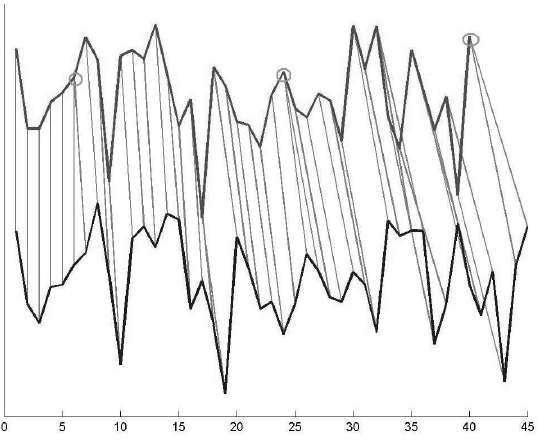
\includegraphics[width=0.5\textwidth]{./figures/figure}
\caption{A figure example.}
\label{fig:figure_label}
\end{figure}

\section{Section 1}
\label{sec:section1}

\begin{table}
\centering
\caption{A table example}
\begin{tabular}{ c c c c }
\toprule
\textbf{Dataset} & \textbf{Number of samples} & \textbf{Results} & \textbf{Results 2} \\
\midrule                 
  Ini & 1405 & 48 & 9 \\ 
  Mid & 1196 & 52 & 10 \\ 
  Fin & 1629 & 44 & 9 \\ 
  Iso & 1372 & 39 & 8 \\ 
  \bottomrule
\end{tabular}
\label{table:table_ex} 
\end{table}



\section {Nomenclature}

For updating nomenclature run the following commands:

makeindex Thesis-main.nlo -s nomencl.ist -o Thesis-main.nls

makeindex LettersClassification.nlo -s nomencl.ist -o LettersClassification.

\chapter{Summary, Conclusions and Future Work}

\begin{itemize}
\item item 1
\item item 2
\end{itemize}



\bibliographystyle{plainnat}
\bibliography{references}

\appendix

\chapter{Appendix 1}

appendix 1 content...

\cleardoublepage
\newpage
\thispagestyle{empty}
\mbox{}


\includepdf[pages=-]{hebrew_part}
\end{document}
